\documentclass[tikz,border=10pt]{standalone}
\usepackage[T1]{fontenc}
\usepackage{mathpazo}
\usepackage{amsmath,amssymb}
\usetikzlibrary{arrows.meta, positioning, calc, decorations.pathmorphing}

\definecolor{stblue}{HTML}{7B97AD}
\definecolor{rwgold}{HTML}{B8995E}
\definecolor{sage}{HTML}{7A9A7E}
\definecolor{dkbrown}{HTML}{3D3530}
\definecolor{wmgray}{HTML}{7B7067}
\definecolor{cream}{HTML}{F9F6F0}
\definecolor{border}{HTML}{D4C9B8}
\definecolor{terracotta}{HTML}{C47A6A}

\begin{document}
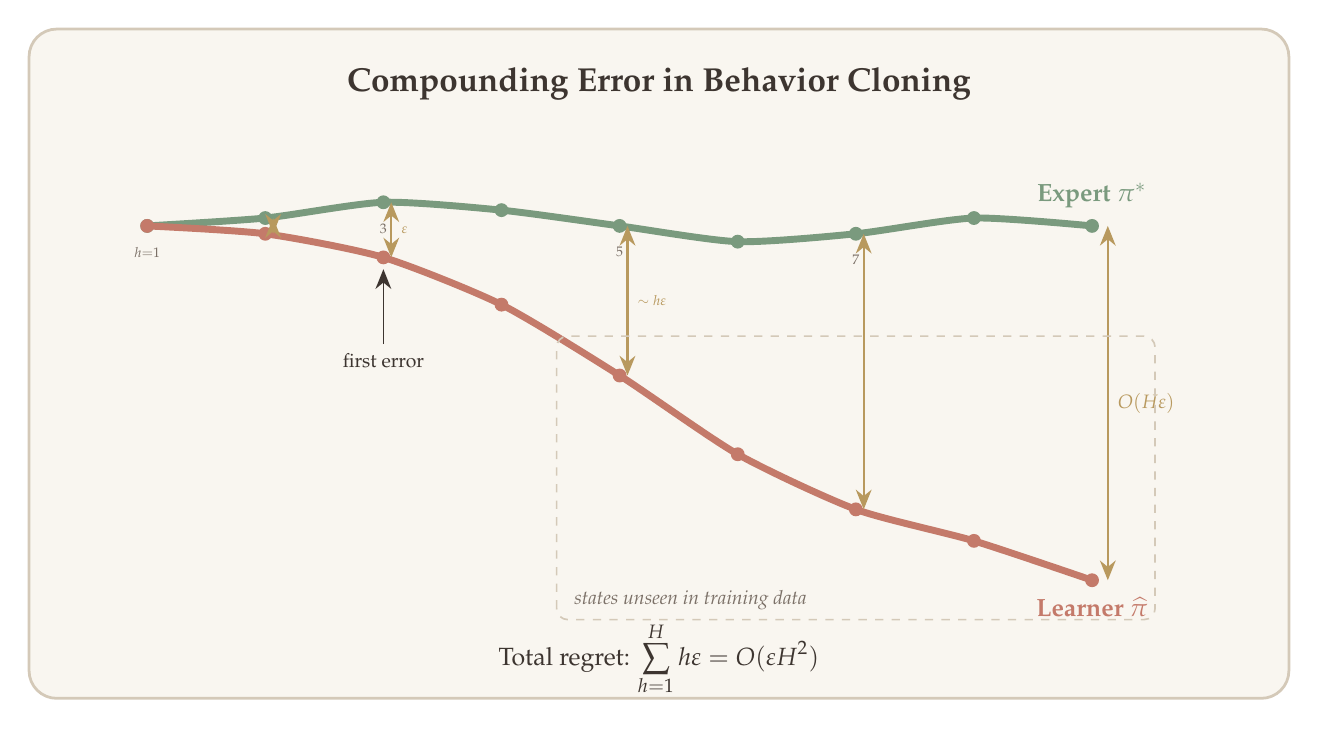
\begin{tikzpicture}[
  >={Stealth[length=2.5mm, width=2mm]},
]

% Background
\fill[cream, rounded corners=10pt] (-1.5,-4.0) rectangle (14.5,4.5);
\draw[border, rounded corners=10pt, line width=1pt] (-1.5,-4.0) rectangle (14.5,4.5);

% Title
\node[font=\large\bfseries, text=dkbrown] at (6.5,3.8) {Compounding Error in Behavior Cloning};

% === Expert trajectory (top, smooth) ===
\draw[sage, line width=2.5pt, smooth, tension=0.4]
  plot coordinates {
    (0.0, 2.0)
    (1.5, 2.1)
    (3.0, 2.3)
    (4.5, 2.2)
    (6.0, 2.0)
    (7.5, 1.8)
    (9.0, 1.9)
    (10.5, 2.1)
    (12.0, 2.0)
  };

% Expert label
\node[font=\small\bfseries, text=sage, anchor=south] at (12.0,2.1) {Expert $\pi^*$};

% Expert state markers
\foreach \x/\y in {0.0/2.0, 1.5/2.1, 3.0/2.3, 4.5/2.2, 6.0/2.0, 7.5/1.8, 9.0/1.9, 10.5/2.1, 12.0/2.0} {
  \fill[sage] (\x,\y) circle (2.5pt);
}

% Step labels along expert
\node[font=\tiny, text=wmgray, below] at (0.0,1.85) {$h{=}1$};
\node[font=\tiny, text=wmgray, below] at (3.0,2.15) {$3$};
\node[font=\tiny, text=wmgray, below] at (6.0,1.85) {$5$};
\node[font=\tiny, text=wmgray, below] at (9.0,1.75) {$7$};

% === Learner trajectory (starts close, drifts away) ===
\draw[terracotta, line width=2.5pt, smooth, tension=0.4]
  plot coordinates {
    (0.0, 2.0)
    (1.5, 1.9)
    (3.0, 1.6)
    (4.5, 1.0)
    (6.0, 0.1)
    (7.5, -0.9)
    (9.0, -1.6)
    (10.5, -2.0)
    (12.0, -2.5)
  };

% Learner label
\node[font=\small\bfseries, text=terracotta, anchor=north] at (12.0,-2.6) {Learner $\widehat\pi$};

% Learner state markers
\foreach \x/\y in {0.0/2.0, 1.5/1.9, 3.0/1.6, 4.5/1.0, 6.0/0.1, 7.5/-0.9, 9.0/-1.6, 10.5/-2.0, 12.0/-2.5} {
  \fill[terracotta] (\x,\y) circle (2.5pt);
}

% === Error arrows showing growing gap ===
\draw[rwgold, line width=0.8pt, <->] (1.6,2.1) -- (1.6,1.9)
  node[midway, right, font=\tiny, text=rwgold] {};
\draw[rwgold, line width=0.8pt, <->] (3.1,2.3) -- (3.1,1.6)
  node[midway, right, font=\tiny, text=rwgold] {$\varepsilon$};
\draw[rwgold, line width=0.8pt, <->] (6.1,2.0) -- (6.1,0.1)
  node[midway, right, font=\tiny, text=rwgold] {$\sim h\varepsilon$};
\draw[rwgold, line width=0.8pt, <->] (9.1,1.9) -- (9.1,-1.6)
  node[midway, right, font=\tiny, text=rwgold] {};
\draw[rwgold, line width=0.8pt, <->] (12.2,2.0) -- (12.2,-2.5)
  node[midway, right, font=\scriptsize, text=rwgold] {$O(H\varepsilon)$};

% === Error annotation at the first deviation ===
\draw[dkbrown, line width=0.6pt, ->] (3.0,0.5) -- (3.0,1.45);
\node[font=\scriptsize, text=dkbrown, align=center, anchor=north] at (3.0,0.5)
  {first error};

% === Region annotation ===
\draw[border, line width=0.6pt, rounded corners=4pt, dashed]
  (5.2,-3.0) rectangle (12.8,0.6);
\node[font=\scriptsize\itshape, text=wmgray, anchor=north west] at (5.3,-2.5)
  {states unseen in training data};

% === Bottom summary ===
\node[font=\small, text=dkbrown, align=center] at (6.5,-3.5)
  {Total regret: $\displaystyle\sum_{h=1}^{H} h\varepsilon = O(\varepsilon H^2)$};

\end{tikzpicture}
\end{document}
